\chapter{选择性符号执行技术}
\label{chap:overview}

\section{符号执行}
\label{sec:sym_exe}

\subsection{基本概念}
\label{sec:original}
符号执行(symbolic execution)使用不确定的符号值(symbolic value)作为输入,将程序中的其他变量值以基于这些符号值的符号表达式(symbolic expression)表示;通过追踪程序中各个可能的执行状态处符号值所需要满足的条件,计算可满足的具体值,将之作为输入带入程序中执行,从而验证在不同的程序输入下程序的正确性。

在程序的任一可能的分叉节点处,符号执行引擎将对应的输入值所需要满足的条件和分支条件进行交运算,之后将该条件交给约束求解器(constraint solver)求解。若条件不可满足,则舍弃该分支结果;否则保留该分支上的路径条件(path condition),将该路径添加到符号执行中。这样,根据每个分支处对条件变量处布尔值的路径条件,在每个分支处可能存在三种情况:
\begin{enumerate}
\item 当仅有True分支条件可满足时,选择True分支
\item 当仅有False分支条件可满足时,选择False分支
\item 当两者的分支上都有可行解时,同时选择Yes和No分支,并添加新的状态
\end{enumerate}
而在选择了的分支处都需要增加对应的条件约束以修正当前路径条件。这里的“分支”在源程序中可能并不存在(存在于源程序中的路径包括分支、循环结构语句等),它们可能是一些隐式的规则约束条件(如被除数不为零、数组元素修改不能因越界导致缓冲区溢出隐患等)。当程序遇到终止条件(正常或异常退出),该程序状态结束;当所有的状态都结束时,符号执行终止。

由于在执行过程中记录了任意程序输入条件下的路径条件,理论上来说通过符号执行验证的程序是正确的。然而一般而言无法通过符号执行工具完整验证程序的正确性。这是因为下面的两个制约:
\begin{itemize}
\item 路径爆炸。符号执行在分支处需要分析程序中所有可满足的执行条件。当遇到循环(或递归)操作时,会考虑循环条件变量导致的所有可能情形,由于条件变量的取值范围有可能很大,符号执行几乎不会达到完全的路径覆盖。
\item 约束求解器的限制。约束求解器总可以求解线性条件约束(尽管未必高效)。然而对于类似于$y=x^3$这样的非线性约束条件在数学上并没有一般的求解方法,符号执行工具必须避免约束求解器求解一般性的非线性约束。同时,对于外部函数调用,约束求解器因为无法得知该函数的具体实现从而不能对其进行约束求解。
\end{itemize}

故在软件测试上,符号执行的目的是在给定的时间限制内执行尽可能多的不同的程序执行路径(execution path):这是由一个\textmd{True}和\textmd{False}组成的序列,在特定程序的位置$i$处的布尔值代表执行路径上第$i$个条件语句的\textmd{then}或\textmd{else}分支。对于每个执行路径需要:
\begin{enumerate}[label={(\arabic*)}]
\item 生成一系列表征该路径条件的具体输入。
\item 检验是否存在断言违反、未捕获异常、安全漏洞或内存中断等错误。
\end{enumerate}

不难发现,和其他分析手段相比,符号执行工具有如下优势:
\begin{enumerate}
\item 从测试的角度,可以自动生成高覆盖率的测试用例。
\item 从寻找程序中bug的角度,由于它提供了可以引发程序错误的具体值,可以脱离符号执行工具来确认程序的错误所在。
\item 和通过动态分析手段对给定的程序路径寻找程序中的错误的方法相比,符号执行工具并不需要给定具体值。
\item 符号执行不仅能找出诸如缓冲区溢出等一般性错误,同时还可以探讨诸如“复杂的断言违反”等语义上的错误。
\end{enumerate}

\subsection{符号执行工具}
\label{sec:tools}

现代的符号执行工具主要面临下述的几个问题:

\subsubsection{路径爆炸}
程序中的路径随着程序规模的扩大往往会急剧增长(path explosion),这使得约束求解器在确定某个条件约束其正、逆条件都能被满足时符号执行器都会添加新的路径条件,这样的增长可能是指数级的。尽管符号执行可以过滤不依赖于符号值的路径或给定当前路径约束条件不可解的路径,对于中大型程序而言执行路径的增长仍然是符号执行的主要瓶颈。这是符号执行本身固有的问题,受限于现代电子计算机的运算能力,理论上没有高效的算法。

然而可以通过一些优化来提高符号执行的速度。
\begin{enumerate}
\item 采用合理的路径选择策略,这可以提高符号执行时的语句覆盖率和分支覆盖率。
\item 当产生新的路径状态时,运用写时复制(copy-on-write)的fork机制,降低产生新状态的开销。
\item 使用具有更强运算能力的计算机。
\end{enumerate}

另一个着眼点在于减少实际符号执行的大小。
\begin{enumerate}
\item 可以通过用户配置提升待验证程序所进行的符号执行的层次,在更高层次上进行符号执行而忽略底层调用。应用程序往往会使用很多高效底层库,在大多数情况下可以认为这些库是正确的;实际中需要验证的是上层应用程序的正确性,故应关注于应用本身。额外对底层库进行符号分析也会带来巨大的开销;同时一些情况下我们无法对库进行符号执行(如建立在源代码层次上的符号执行)。
\item 仅验证部分可能的程序错误。程序中会遵循一些特定的规则,违反这些规则会使得程序存在潜在的错误;可以将符号执行仅应用于这些和规则相关的路径上而在另外一些路径正常执行。也可以结合静态分析的方法实现削减那些不相关的路径以简化程序输入。
\end{enumerate}

\subsubsection{约束求解器的局限}
\label{sec:solver_restrict}

符号执行过程中的路径条件的计算是依赖于约束求解器(constraint solver)的,约束求解器的性能直接关系到符号执行的优劣。事实上,统计数据表明,符号执行中约束求解占据了大量的时间:在不含任何优化的情况下,求解约束条件花费的时间可能占$90\%$以上~\upcite{KLEE}。然而,不同的约束求解器有不同的特性,同时亦取决于查询约束的种类以及和符号执行引擎的结合方式,这使得现代的约束求解器有相当复杂的配置条件。一般而言,约束求解器往往只能处理好线性整形约束;尽管有不少工具将浮点型也作为约束条件,但是收效并不明显;不少理论研究正着眼于解决这一问题。为减轻约束求解器的负担,符号执行引擎可以提供一些优化。
\begin{enumerate}
\item 对输入程序本身进行编译优化。
\item 不相关约束削减。由于大部分程序分支可能仅依赖于很少的变量,而减少约束求解的维度可以大大加速约束求解器的求解。
\item 缓存可行解。将每次由约束求解器计算得到的结果保存下来,当需要求解后续约束条件时,首先在已有的具体值缓存中查看是否满足条件约束,仅当无可行解时才交由约束求解器求解。
\end{enumerate}

\subsubsection{存储建模(memory modeling)}
不同的存储模型对符号执行器的精确性影响很大。如使用定点数(fixed pointer number)并不能完整刻画语句的状态值(整型等类型都有一定的范围),在遇到指针变量时选择具体值而不再使用符号值会有不少结果可满足的条件被错误地忽略了,将系统运行库带入符号执行系统与否也会给符号执行状态造成不同的结果(部分符号执行引擎在遇到外部函数调用的时候往往会使用具体值而不是符号值带入执行)。

\subsubsection{处理并发程序}
\label{sec:concurrency}

大型的并发程序由于不再具有顺序性而带来了不确定的因素,对这样的程序的测试相当困难,同时在并发程序上进行符号执行也是一大挑战。

\subsection{工作流程}
\label{sec:tool}

如前所述,符号值在循环或递归时会产生很多路径,往往耗费大量的时间;研究人员经常在符号执行器运行时给单个语句(或指令等,视具体实现情景而定)设定最长运行时间或最大运行深度。这也会造成一些不精确,然而这在现实中是可以接受的。同样地,对约束求解器而言,符号执行时通常也会给定一个时间或深度上的限制。由此说来,现代已实现的符号执行引擎并不能保证程序的正确性;但是在检测程序中含有错误方面,它们仍然比软件测试、静态分析等手段要高效得多,这使得这方面的研究正越来越受到关注。

现代符号执行引擎的工作流程如\autoref{fig:se_workflow}所示。通常先将待测程序\patch 转化为中间表达形式(IR),再在其基础上对该中间形式作适当转化得到符号执行引擎可以理解的程序片段,最终根据不同的解释方法进行符号执行生成测试用例。这里的\patch 依据符号执行工具的特性可以是源代码形式或不同平台下的二进制形式。
\begin{figure}[t]
\begin{center}
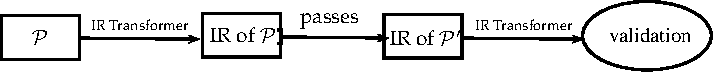
\includegraphics[width=.9\textwidth]{fig/se_workflow.pdf}
\bicaption[fig:se_workflow]{符号执行工具的整体工作流程}{符号执行工具的整体工作流程}{Fig}{Overall Workflow of a typical Symbolic Execution Tool}
\end{center}
\end{figure}

\section{KLEE简介}
\label{sec:llvm_klee}

\subsection{LLVM分析框架}
\label{sec:llvm}
LLVM的原意是底层虚拟机(Low Level Virtual Machine),是一个编译器基础框架,它提供了一种几乎和机器无关的中间表达形式(Intermediate Representation, IR或bitcode),使得任意程序语言只要可以表达成该形式都可以使用LLVM的分析框架进行优化。由于LLVM的中间表达形式将编译器前端和LLVM后端完整分离开来,只要满足LLVM的IR规约就可以生成正确的中间代码,这大大统一了分析的方法,降低了分析的门槛。同时,LLVM良好的设计使得在编译时期、链接时期、运行时期以及“闲置时期”都可以进行优化。符号执行引擎KLEE正是基于LLVM提供的这些特性才得以成为现实。越来越多的学者进行这方面的研究,基于LLVM的研究使得程序语言领域、软件工程方面取得的进展突飞猛进。

LLVM的中间表达形式语义极其丰富,可以支持ActionScript, Ada, D, Fortran, GLSL, Haskell, Java 字节码, Julia, Objective-C, Python, Ruby, Rust, Scala 和 C\#等多种语言。我们可以使用对应的前端工具如llvm-gcc,clang,dragonegg,llgo来使得生成对应的IR。LLVM提供了各种工具对这一中间表达形式进行分析、转化,如llvm-dis(中间代码反编译)/llvm-as(中间代码序列化),opt(中间代码优化)等;同时我们可以使用LLVM的API方便地编写LLVM的扩展应用,\dryrun 正是基于llvm的opt工具和其提供的分析、转化的API之上的。

\subsection{KLEE系统}
\label{sec:klee}

KLEE是建立在LLVM框架上的符号执行系统,出现于2008年,在2009年正式开源。具体说来,相比较以往的符号执行工具,KLEE有以下优势:
\begin{enumerate}
\item 对程序本身做了一些基于LLVM框架的编译优化(如常量传递、死代码消除等),简化待验证程序。
\item 结合了启发式路径探寻方法、约束集削减方法以及约束查找缓存机制,在很大程度上减少了约束求解器STP的查询次数。
\item 对内存进行了细粒度建模,利用了LLVM中间表达形式的扩展性,保证了程序执行状态的准确性。
\item 为了提高性能,它还利用了posix的底层fork机制,使得程序状态开销大大减少。
\item 提供了C的库函数$\mu clibc$的链接,使得通过一定的配置可以对文件、IO等底层函数符号化。
\end{enumerate}

KLEE的这些做法使得它适合处理偏向底层的程序,在对coreutils的89个工具测试中,在没有人工参与的情况下KLEE花费89小时生成的测试用例比15年来人工编写测试用例的覆盖率还高,同时找出了这些工具中被忽视多年的程序错误。这一结果使得人们意识到符号执行完全可以胜任特定系统环境下的测试用例集生成和错误检测。

\section{术语简介}
\label{sec:term}
为方便论述,首先介绍在\nameref{chap:symb}中提到的符号。
将原先的错误版本程序记为\bug ,而经过修改过的程序记为\patch ,一般意义下的程序使用\prog 来代指。如无特别说明,这3个符号的含义是宽泛的:既可以指代不加修改的源程序,也可以指代程序中的经过转化过的中间代码形式。

对于某一特定程序,将\prog 的出错位置(bug site)记为\prog\bs ,而把修改的补丁位置(可为多处)记为\prog\ps 。下面将会提到,\dryrun 所考虑的\prog\bs 都是程序中可能转化为断言的地方(assertion) \prog\ass ,故在源代码层次上,可以认为\prog\ass 和\prog\bs 都指的是assert宏的调用处(在C代码中一般会扩展为$\_\_assert\_fail$函数调用),后文将不加地区分使用这两者。\prog\bs 是导致程序执行时触发断言的根源程序片段,在实际中代指\bug 和\patch 中修改的代码对应的所在\bug 或\patch 中的那部分代码。和\prog\bs 不同,\prog\ps 可以为在代码上(源代码层次或中间层次)不连续的多个包含位置信息的代码片段(或仅为占位符性质的空操作)。若赋予程序中的语句以位置信息,在同一层次(可以是源代码或中间形式,也可以是经过若干步相同的优化后的代码)的转化下有等式\ref{eq:1}。
\begin{equation}
  \label{eq:1}
  (\bug \setminus \bug\ps )\cup \patch\ps = \patch
\end{equation}

程序的\rbscope 是\prog 的一个(非严格意义上的)子集,它包含了以指定的函数为执行入口,所有可能被执行到的程序相关代码片段。这样的\rbscope 有如下三种不同的精确程度:
\begin{enumerate}
\item 基于未被调用函数的削减结果。在指定了程序的入口函数之下,不少函数不会被调用到,在这种情况下可以首先剔除那些不会被调用的函数。这时的程序削减是依赖于调用图以函数为粒度的,得到的\rbscope 是\prog 的严格子集。
\item 基于基本块(Basic Block)可达性上的削减结果。该削减可能会额外添加含有不影响相关所关注路径语义的语句。
\item 基于对\prog\bs 影响性分析上的削减。同样,该削减会添加额外的语义以使得削减结果符合语法。
\end{enumerate}

对于某个程序\prog ,将其\rbscope 记为\prog\scope 。由于所做改动可能会导致数据流
和控制流及指向上较大的变化,\bug\scope 和\patch\scope 会有很大差异,并不能保证述等式\ref{eq:2}成立。
\begin{equation}
\label{eq:2}
(\bug\scope \setminus \bug\ps )\cup \patch\ps = \patch
\end{equation}

\section{一个典型例子}
\label{sec:gimp_example}

\autoref{fig:example} 展示了一段摘自GIMP 2.6.11\footnote{GIMP: GNU Image Manipulation Program, http://www.gimp.org/} Paint Shop Pro(PSP)插件简短的代码片段。图中以横线划去的部分为初始的不完整补丁,绿色的行为最终的正确补丁,而灰色的编辑行是通过\dryrun 的削减技术判断可以被删除的部分。当一个通过RLE压缩的PSP\_COMP\_RLE图像文件(第1行)在图像结束处{\tt runcount}(第7行)取值很大时,在第18行或者24行会发生基于堆的缓冲区溢出\footnote{https://bugzilla.gnome.org/show\_bug.cgi?id=639203.}。这一bug可能会被远程入侵者用于拒绝服务(DoS,denial of service)攻击,进一步可能被用于执行任意恶意代码。对该bug的第一个修改补丁位于第15行\footnote{https://abf.rosalinux.ru/fresh/gimp/blob/master/gimp-2.6.11-psp-overflow.patch}。然而该补丁是不完整的,它仅仅将第18行的bug修补了,第24行的断言仍然有可能被触发。这个问题于四个月之后第二次在CVE-2010-4543中被重新提出\footnote{http://web.nvd.nist.gov/view/vuln/detail?vulnId=CVE-2010-4543},最终有人给出了位于第16行的另一个补丁才终于将它修复。

如果程序员可以对第一次修改过的补丁程序进行验证,分析出\texttt{bytespp}和 \texttt{runcount}所有可能的取值,则可以避免这一不完全的补丁。然而,完全的补丁验证相对而言殊非易事(而对这一特例的补丁验证更为困难)。考虑到GIMP中有数百万的代码,普通的程序测试手段通常不能对该补丁进行完整测试,这是由于程序的规模增大导致了路径和程序状态以指数级增长。注意到第15行的程序相对较小,并且局限于修复第18行和第24行处的错误,如果将程序的关注范围局限于由补丁处至出错点处的部分,则可以大大减小待测程序片段的大小,因此可以对此使用规模相对较小然而更为完整的符号执行。我们给出了通过有选择性的符号执行来进行完整并快速的补丁验证的系统\dryrun 。

\begin{figure}[t]
\begin{center}
\begin{lstlisting}[language={[ANSI]C}]
%* \color{mygray}{case PSP\_COMP\_RLE: { } *)
  %* \color{mygray}{q = pixels[0] + offset;} *)
  %* \color{mygray}{endq = q + npixels * bytespp; } *)
  %* \color{mygray}{buf = g\_malloc (127); } *)
  while (q < endq) {
    %* \color{mygray}{p = buf; } *)
    fread (&runcount, 1, 1, f);
    if (runcount > 128) {
      runcount -= 128;
      %* \color{mygray}{{fread ($\&$byte, 1, 1, f); }} *)
      %* \color{mygray}{{memset (buf, byte, runcount); }} *)
    %* \color{mygray}{{\} else }} *)
      %* \color{mygray}{{fread (buf, runcount, 1, f); }} *)
      %* \color{mygray}{{/* prevent buffer overflow for bogus data*/ }} *)
      %* \sout{\texttt{runcount = MIN(runcount, endq - q);}} *)
      %* \color{mygreen}{\texttt{runcount = MIN(runcount, (endq-q)/bytespp);}} *)
      if (bytespp == 1) {
        assert (q + runcount < endq);
        %* \color{mygray}{{memmove (q, buf, runcount); }} *)
        q += runcount;
      } else {
        %* \color{mygray}{\texttt{p = buf;}} *)
        for (i = 0; i < runcount; i++) {
          assert (q < endq);
          %* \color{mygray}{{*q = *p++; }} *)
          q += bytespp;
        }
      } }
    %* \color{mygray}{{g\_free (buf); break; }} *)
\end{lstlisting}
\vspace{-0.5cm}
\bicaption[fig:example]{一个选择性符号执行的例子}{一个选择性符号执行的例子}{Fig}{An Illustrating Example for Selective Symbolic Execution}
\end{center}
\end{figure}


\section{\dryrun 的工作流}
\label{sec:dryrun_workflow}

\begin{figure}[t]
\begin{center}
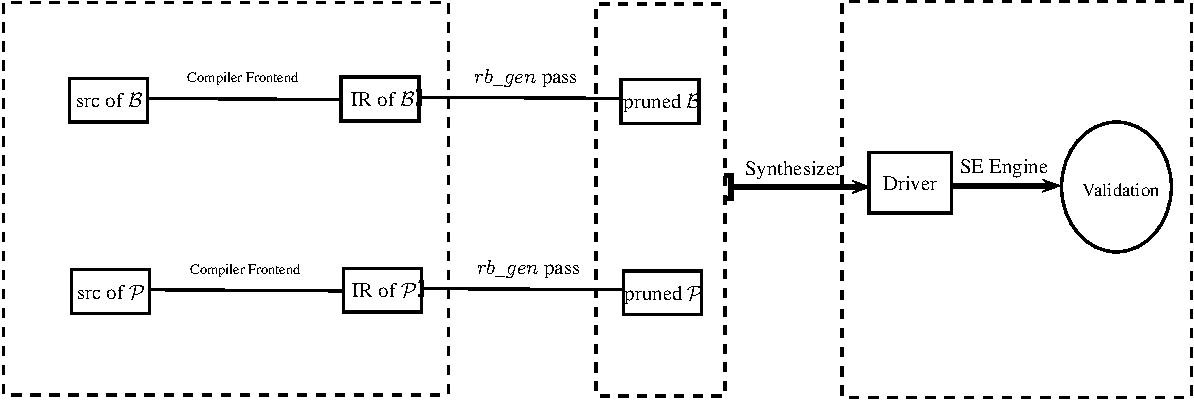
\includegraphics[width=\textwidth]{fig/workflow.pdf}
\bicaption[fig:workflow]{\dryrun 的整体工作流程}{\dryrun 的整体工作流程}{Fig}{Overall Workflow of \dryrun}
\end{center}
\end{figure}

\autoref{fig:workflow}展示了\dryrun 原理。和\autoref{fig:se_workflow}相比,不难看出\dryrun 的原创之处在于中间代码的转化上,并且使用两个版本程序经过添加程序驱动得以进行符号执行。

\noindent\textsf{定位程序\prog 的出错节点\prog\bs 和补丁节点\prog\ps\quad } 
\dryrun 首先根据源代码上的行号、变量名等信息确定程序配置程序的\prog\ps 及\prog\bs 。这里,\dryrun 主要关注的错误为程序中断言违反或可以转化为断言违反的缓冲区溢出或程序崩溃,对于C代码而言这是很常见的错误。另外,我们假设\prog\ps 是以差异(diff)文件为表现形式的,这可以从git、svn等源代码版本控制系统(version control system)管理的代码中非常方便地得到。因此,对程序\prog 的错误节点\prog\bs 及补丁节点\prog\ps 的定位是直接的:程序发生错误的节点所在语句被认为是\prog\bs,而修改(相对于原有的代码可能是添加、修改、删除一处或多处)的语句集合被认为是\prog\ps 。在\autoref{fig:example}这一例子中,第16行和第24行为\prog\bs ,而第15行为\prog\ps 。实际情形中,\prog\ps 和\prog\bs 都可能包含多个代码编辑行,在{\autoref{sec:complex}}将会提到如何对这一问题进行处理。

\noindent\textsf{程序中的极小有界区域的计算\quad} 
把\prog 的\prog\ps 和\prog\bs 作为输入,通过静态分析的方法,\dryrun 选取了补丁程序中的极小(minimal)部分(该部分即为\rbscope);这是通过三种不同粒度上的削减完成的。

首先依据上下文不敏感(context insensitive)的Andersen指向(points-to)算法,对程序的编译单元得到指向结果的概要(summary);在此基础之上,建立程序的精确调用图(call graph)信息,并得到函数调用点处(call site)处对变量的修改信息。至此,完成了基础的分析。之后,依据上述分析结果,对程序做未调用削减、基于可达性的削减及基于程序影响性分析的削减。

给定程序的入口函数,编译单元中存在一些未被调用的函数;这些函数虽然不会影响到最终的符号执行,但是会增加后期指向分析的复杂性,并且使得最终削减结果不够精确。基于此的削减是仅依赖程序的调用图信息。

对于由补丁处及错误处决定的程序片段,通过静态分析可以得到程序中的一些不可能被执行到的片段——这可以归结为程序的过程间控制流图(inter-procedural Control Flow Graph)的图可达性问题,将由程序补丁处不可达到的程序基本块(basic block)或不可到达程序出错处的基本块在保证关心路径语义正确的前提下进行削减。

程序的可达性分析并不能进一步削减程序中那些可达出错处但不会影响到该出错处的程序,对这些程序片段的削减是通过程序后向切片(backward slicing) (参见\ref{sec:slicing}) 完成的。涉及到的算法是基于不动点的,故最终削减结果并不唯一~\upcite{Slicing81};故而该有界区域是极小的而非最小。

\noindent{\textsf{生成验证驱动程序}\quad}
\dryrun 需要给\rbscope 添加上入口函数及符号执行的语义,使得可以被对应的符号执行引擎所理解。

对于上述例子\autoref{fig:example}的驱动程序,其结果如\autoref{fig:example_result}所示。其中合成器在第1至3行添加了变量的定义,并符号化未定义变量(第21行),同时程序员添加一些额外的前置条件(如第22行所示,具体参见\autoref{sec:user_init}), 进一步将\rbscope 封装在一个函数 $patch\_rbscope$中(第4至19行)。

\noindent{\textsf{基于符号执行的补丁验证}\quad} 
最终将所合成的驱动程序交由符号执行引擎进行执行。符号执行的分析工具保留当前的路径条件并由求解器计算出其所有可行结果条件,之后检测到程序出错路径是否可解。若路径可解,\dryrun 会警告这是一条不正确的路径;反之,认为该执行路径是正确的。

\noindent{\textsf{交叉验证}\quad}
为更进一步探究不正确的补丁程序是不完整的或引发了新的程序错误,\dryrun 还对原错误程序及补丁程序的执行作了比较。这一过程需要将两个版本的程序同时融合于一个编译单元中,并向原有的程序驱动中添加交叉验证的操作语义。这使得可以在更精确的路径粒度上对不同版本程序进行分析。

\begin{figure}[t]
\begin{center}
\begin{lstlisting}[ basicstyle=\ttfamily\bfseries\footnotesize, language={[ANSI]C}]
char *buf, *q, *endq;
unsigned int bytespp, runcount;
FILE *f;
patch_rbscope() {
  while (q < endq) {
    fread(&runcount, 1, 1, f);
    if (roncount > 128)
      runcount -= 128;
    runcount = MIN(runcount, (endq-q)/bytespp);
    if (bytespp == 1) {
      assert (q + runcount < endq);
      q += runcount;
    } else {
      for (int i = 0; i < runcount; i++) {
        assert (q < endq);
        q += bytespp;
      }
    } }
}

int main(void) {
  make_symbolic(&q, &endq, &bytespp, &f);
  assume(q < endq);
  patch_rbscope();
}
\end{lstlisting}
\vspace{-0.5cm}
\bicaption[fig:example_result]{对\autoref{fig:example} 生成的驱动程序}{对\autoref{fig:example} 生成的驱动程序}{Fig}{Generated driver program for \autoref{fig:example}}
\end{center}
\end{figure}

\section{本章小结}
\label{sec:c2}
本节主要介绍了\dryrun 所使用的选择性符号执行中涉及到的一些技术。首先介绍了符号执行的基本概念,并分析了影响符号执行扩展性的几个挑战;接下来简单介绍了\dryrun 所基于的LLVM框架及符号执行工具KLEE。在给出了\nameref{chap:symb}中符号的表示意义之后,通过一个具体的例子,解释\dryrun 的具体工作流程。